\let\negmedspace\undefined
\let\negthickspace\undefined
\documentclass[journal]{IEEEtran}
\usepackage[a5paper, margin=10mm, onecolumn]{geometry}
%\usepackage{lmodern} % Ensure lmodern is loaded for pdflatex
\usepackage{tfrupee} % Include tfrupee package

\setlength{\headheight}{1cm} % Set the height of the header box
\setlength{\headsep}{0mm}     % Set the distance between the header box and the top of the text

\usepackage{gvv-book}
\usepackage{gvv}
\usepackage{cite}
\usepackage{amsmath,amssymb,amsfonts,amsthm}
\usepackage{algorithmic}
\usepackage{graphicx}
\usepackage{textcomp}
\usepackage{xcolor}
\usepackage{txfonts}
\usepackage{listings}
\usepackage{enumitem}
\usepackage{mathtools}
\usepackage{gensymb}
\usepackage{comment}
\usepackage[breaklinks=true]{hyperref}
\usepackage{tkz-euclide} 
\usepackage{listings}
% \usepackage{gvv}                                        
\def\inputGnumericTable{}                                 
\usepackage[latin1]{inputenc}                                
\usepackage{color}                                            
\usepackage{array}                                            
\usepackage{longtable}                                       
\usepackage{calc}                                             
\usepackage{multirow}                                         
\usepackage{hhline}                                           
\usepackage{ifthen}                                           
\usepackage{lscape}
\usepackage{circuitikz}


\author{EE25BTECH11041-Naman Kumar }
\graphicspath{./figs/}

\begin{document}
\begin{center}
    \huge{2.10.69}\\
    \large{EE25BTECH11041 - Naman Kumar}
\end{center}
Question:\\
Determine the value of c so that for all real x, the vector $cx\hat{\imath}-6\hat{\jmath}-3\hat{k}$ and $x\hat{\imath}+2\hat{\jmath}+2cx\hat{k}$ make an obtuse angle with each other.\\
\solution \\
We know, Inner Product of two vectors
\begin{align}
    \vec{A}^T\vec{B}=\lVert\vec{A}\rVert\lVert\vec{B}\rVert \cos{\theta}
\end{align}
for obtuse angle between any two vectors
\begin{align}
\cos{\theta}<0\text{ or } \vec{A}^T\vec{B}<0
\end{align}
Given Vectors
\begin{align}
    \vec{A}=\begin{pmatrix}cx\\-6\\-3\end{pmatrix},
    \vec{B}=\begin{pmatrix}x\\2\\2cx\end{pmatrix}
\end{align}
Now using these condition on given vectors
\begin{align}
\vec{A}^T\vec{B}<0\\
\begin{pmatrix}cx&-6&-3\end{pmatrix}\begin{pmatrix}x\\2\\2cx\end{pmatrix}<0\\
cx^2-12-6cx<0\text{ ( quadratic in x)} \label{quad}
\end{align}
for any quadratic to be negative $\forall x \in R$, their are two conditions
\begin{align}
    a<0 \&D<0\\
\end{align}
Now applying this conditions on \eqref{quad}
firstly on a (leading coefficient)
\begin{align}
    c<0 \label{1}
\end{align}
on D (discriminant)
\begin{align}
    D=b^2-4ac<0\\
    (-6c)^2-4\times c \times(-12)<0\\
    36c^2+48c<0\\
    c(3c+4)<0 \label{2}
\end{align}
therfore, by taking union of \eqref{1} and \eqref{2} 
\begin{align}
    c\in(\frac{-4}{3}, 0)
\end{align}
\newpage
\begin{figure}[H]
    \centering
    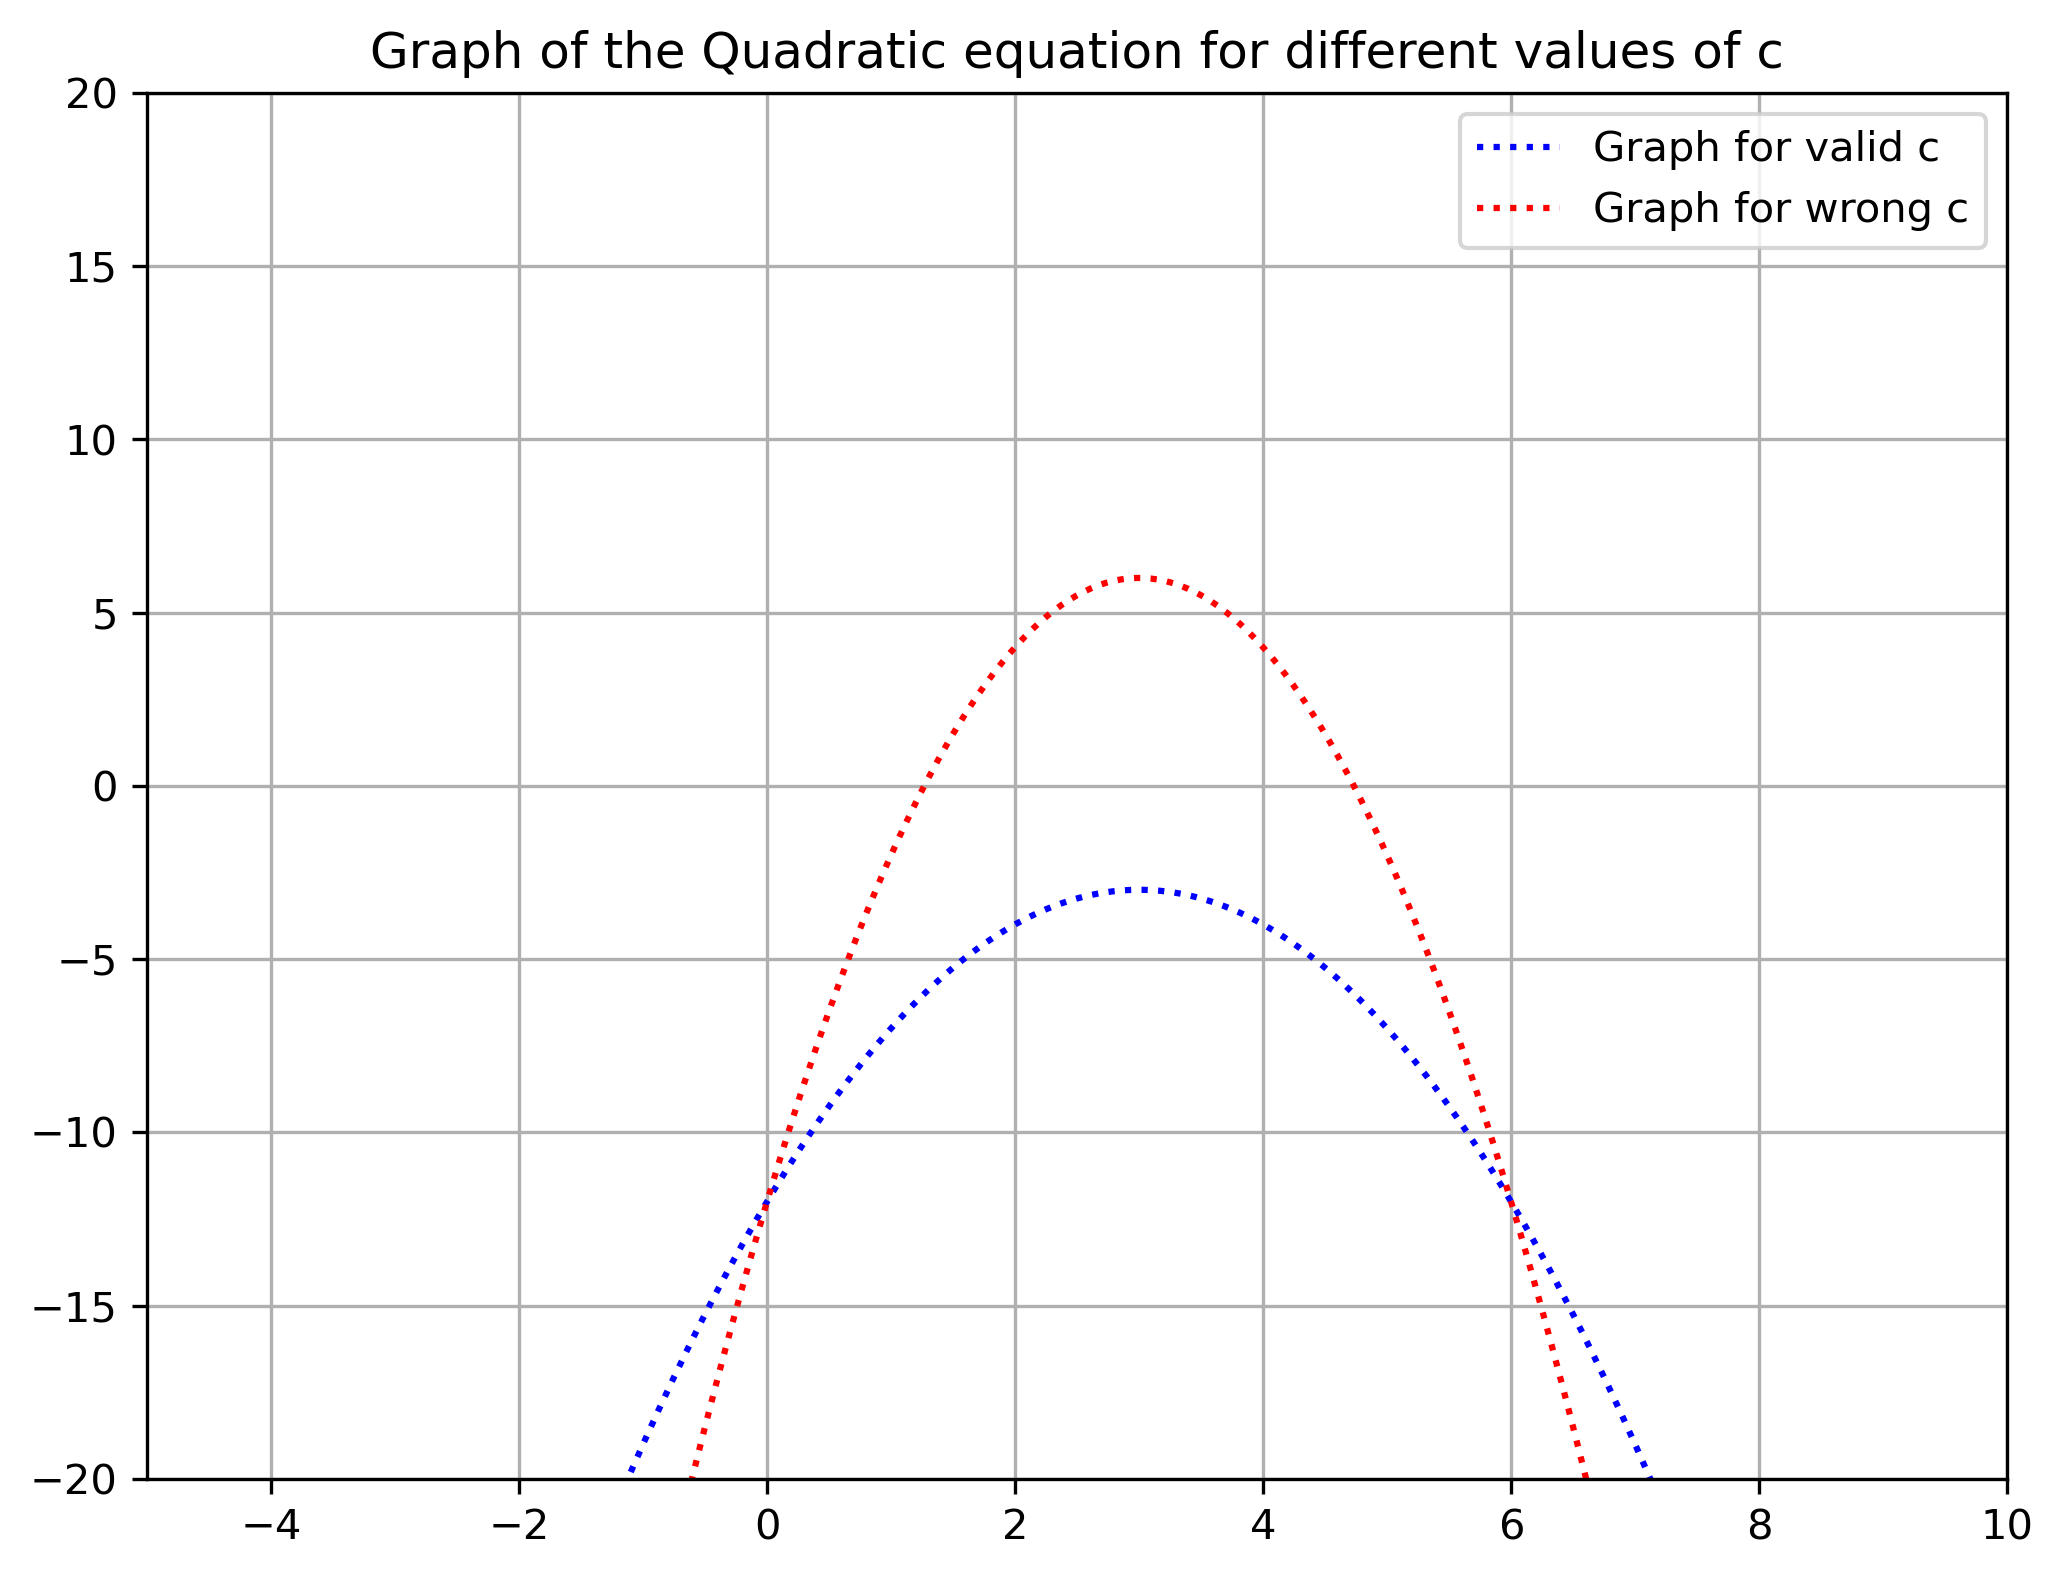
\includegraphics[width=\columnwidth]{figs/figure.png}
    \label{fig:placeholder}
\end{figure}
\end{document}
